\documentclass{article}
\usepackage[utf8]{inputenc}
\usepackage{graphicx}
\begin{document}

\section{Bisection algorithm for simplical meshes}
\label{sec:title}

\begin{itemize}
	\item Serial algorithm
	\item Longest edge splitting with propagation front
	% \item Local refinement propagation so that the levels of refinement of the one-ring
	% neighbors it differs at most one.
	\item For 2D meshes with triangles isosceles the number of congruence classes is 1. 
	\item The algorithm works directly for 3D and 4D.
\end{itemize}

\begin{figure}[htbp]
	\centering
	\parbox{0.5\linewidth}{
	
\includegraphics[width=0.32\linewidth]{figures/mesh_2_bisect_1} \hfill
	
\includegraphics[width=0.32\linewidth]{figures/mesh_2_bisect_2} \hfill
	
\includegraphics[width=0.32\linewidth]{figures/mesh_2_bisect_3} \par
	
\includegraphics[width=0.32\linewidth]{figures/mesh_2_bisect_4} \hfill
	
\includegraphics[width=0.32\linewidth]{figures/mesh_2_bisect_5} \hfill
	
\includegraphics[width=0.32\linewidth]{figures/mesh_2_bisect_6} \par
	
\includegraphics[width=0.32\linewidth]{figures/mesh_2_bisect_7} \hfill
	
\includegraphics[width=0.32\linewidth]{figures/mesh_2_bisect_8} \hfill
	
\includegraphics[width=0.32\linewidth]{figures/mesh_2_bisect_9} \par
	}
	\caption{Steps of the bisection algorithm.}
	\label{fig:two_dim}
\end{figure}

\begin{figure}[htbp]
	\centering
	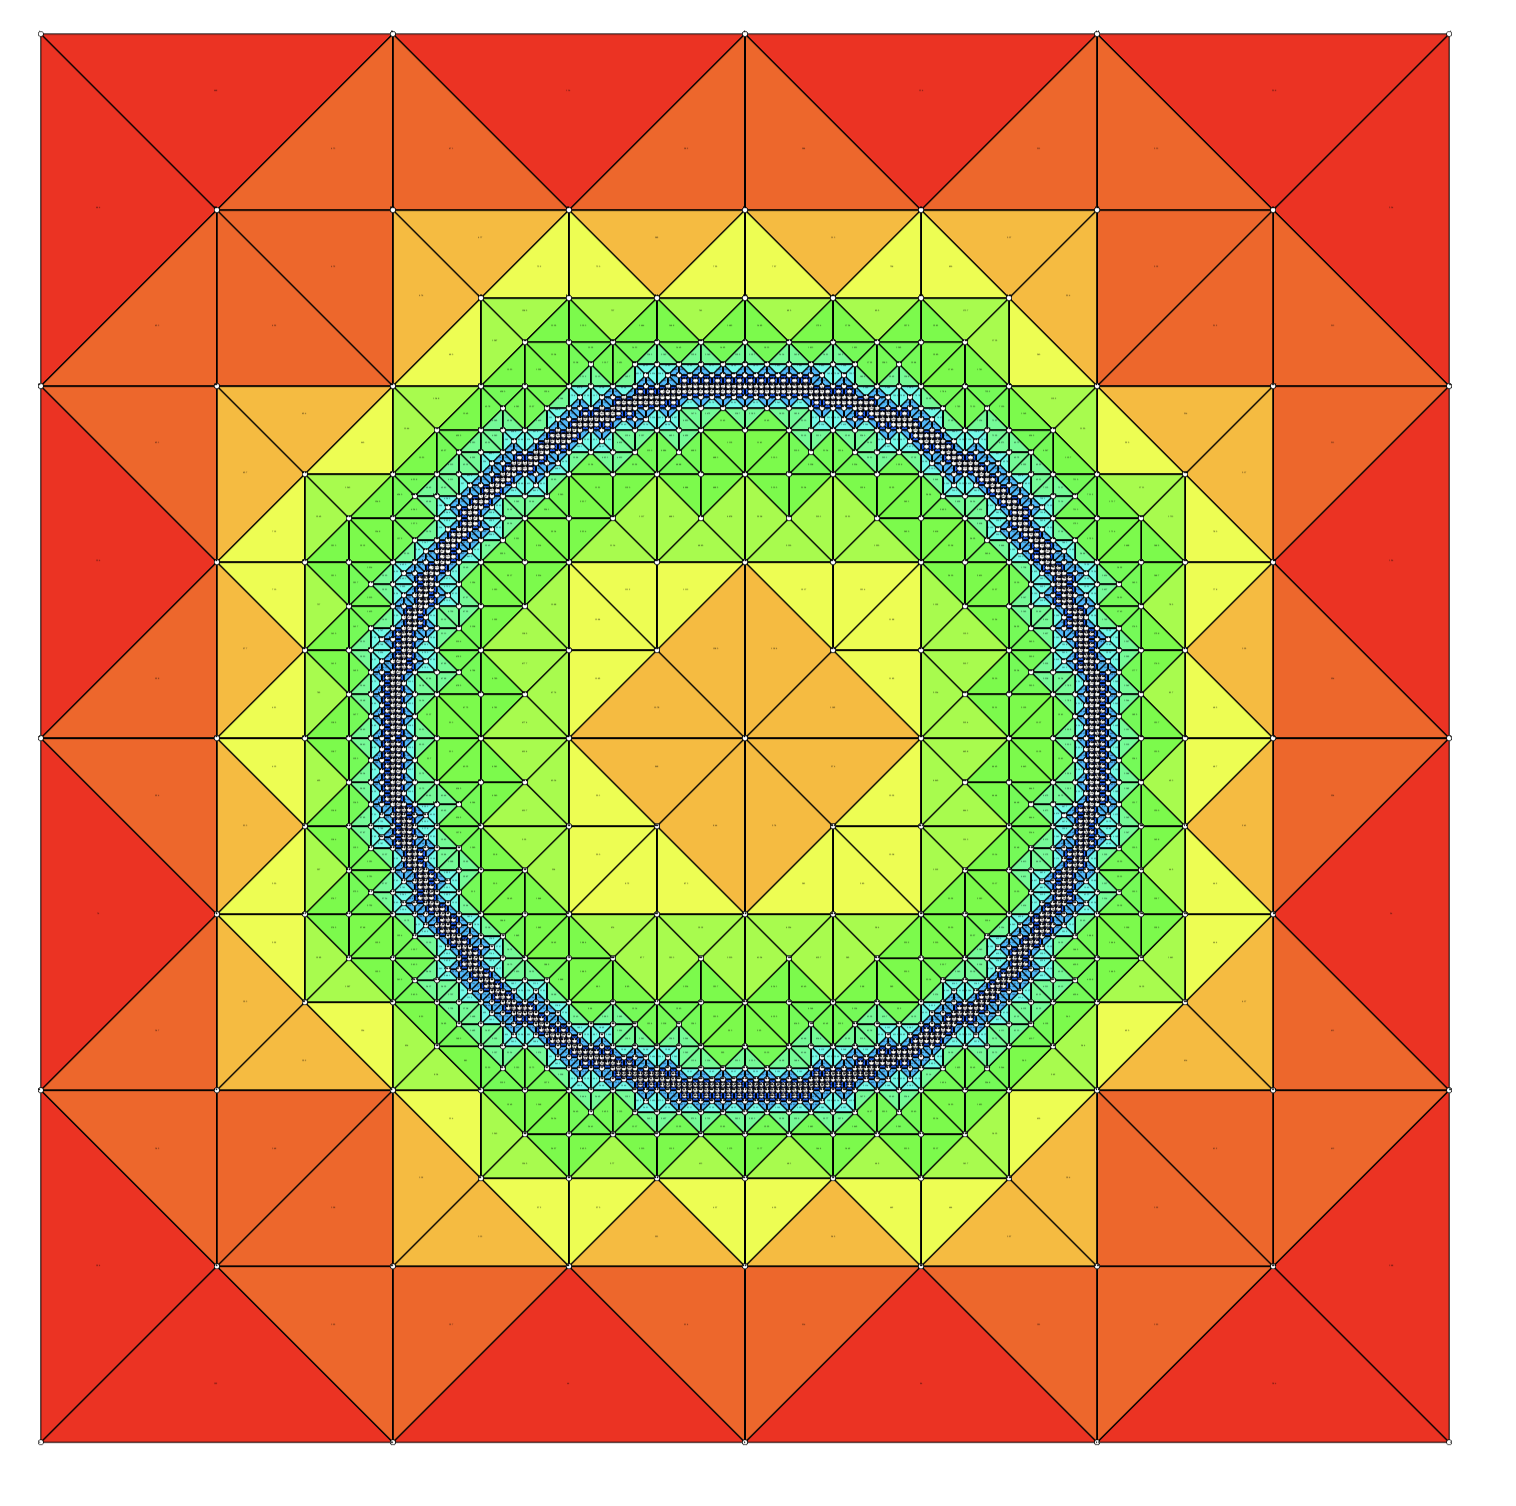
\includegraphics[width=0.40\linewidth]{figures/2d_sphere} \hfill
	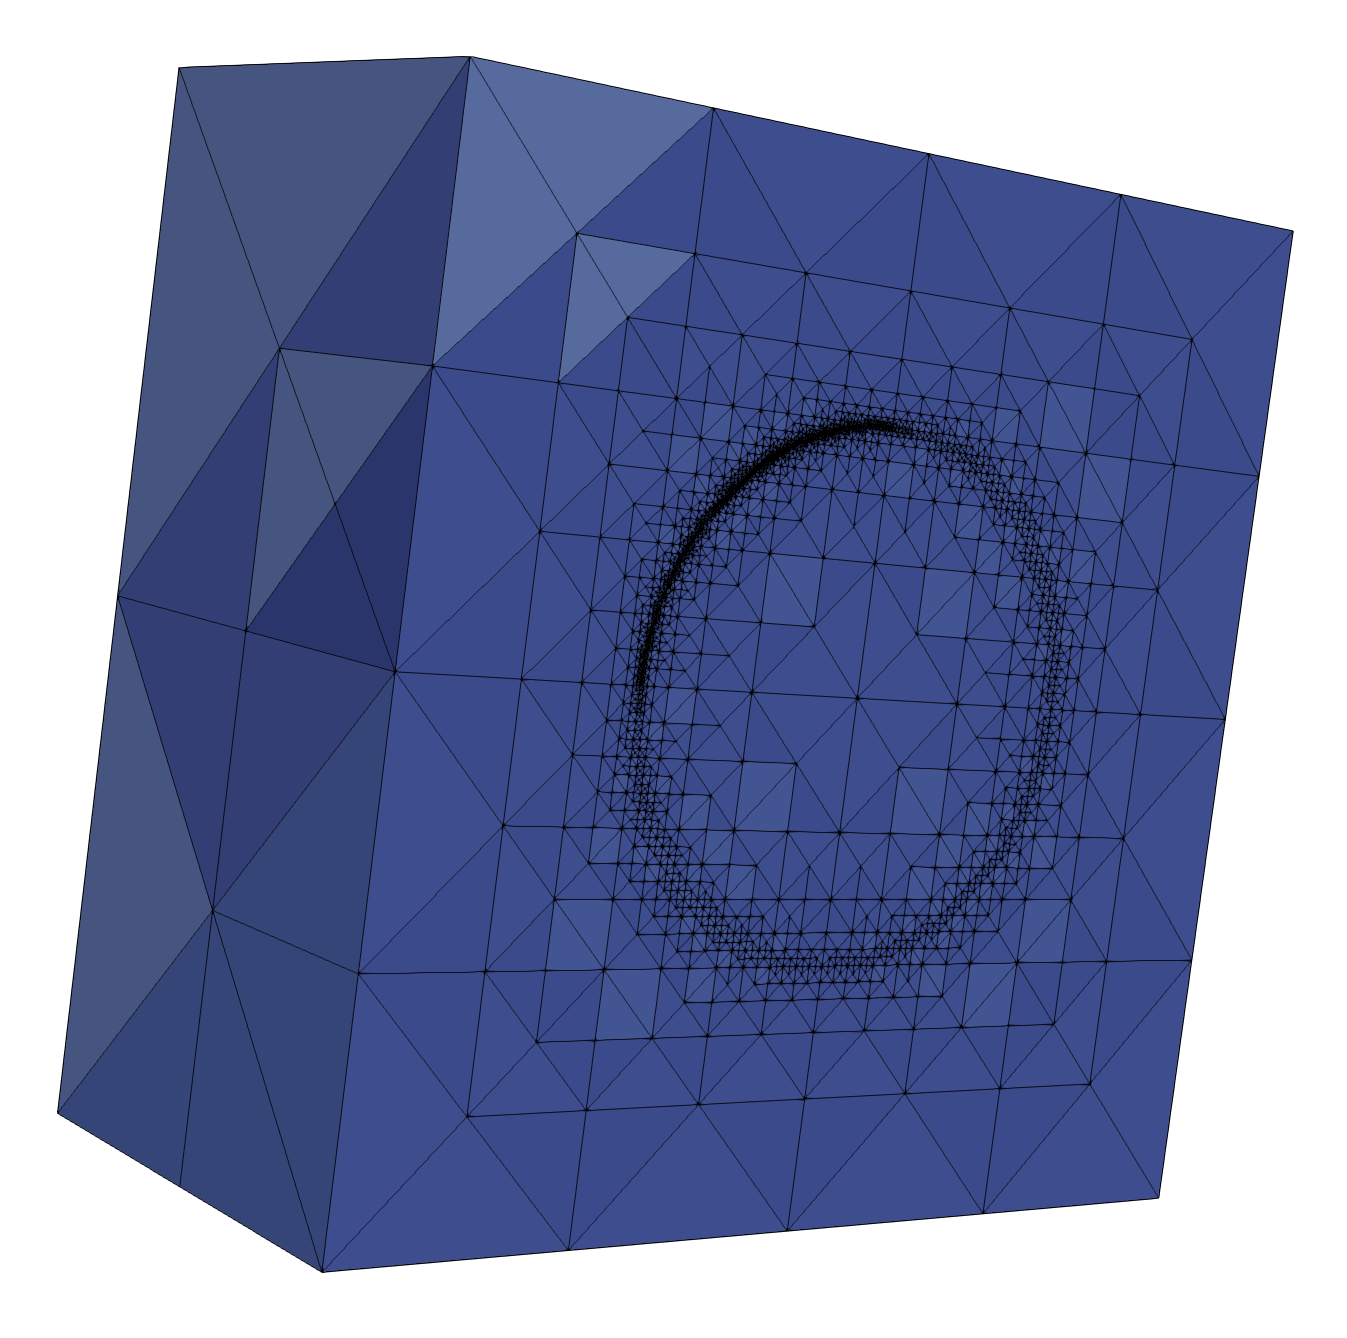
\includegraphics[width=0.40\linewidth]{figures/3d_sphere} 
	\caption{Result for sphere refinement pattern. Left: 2D. Right: 3D.}
	\label{fig:sphere}
\end{figure}

\section{Quality for recursive longest-edge}

\begin{figure}[htbp]
	\centering
	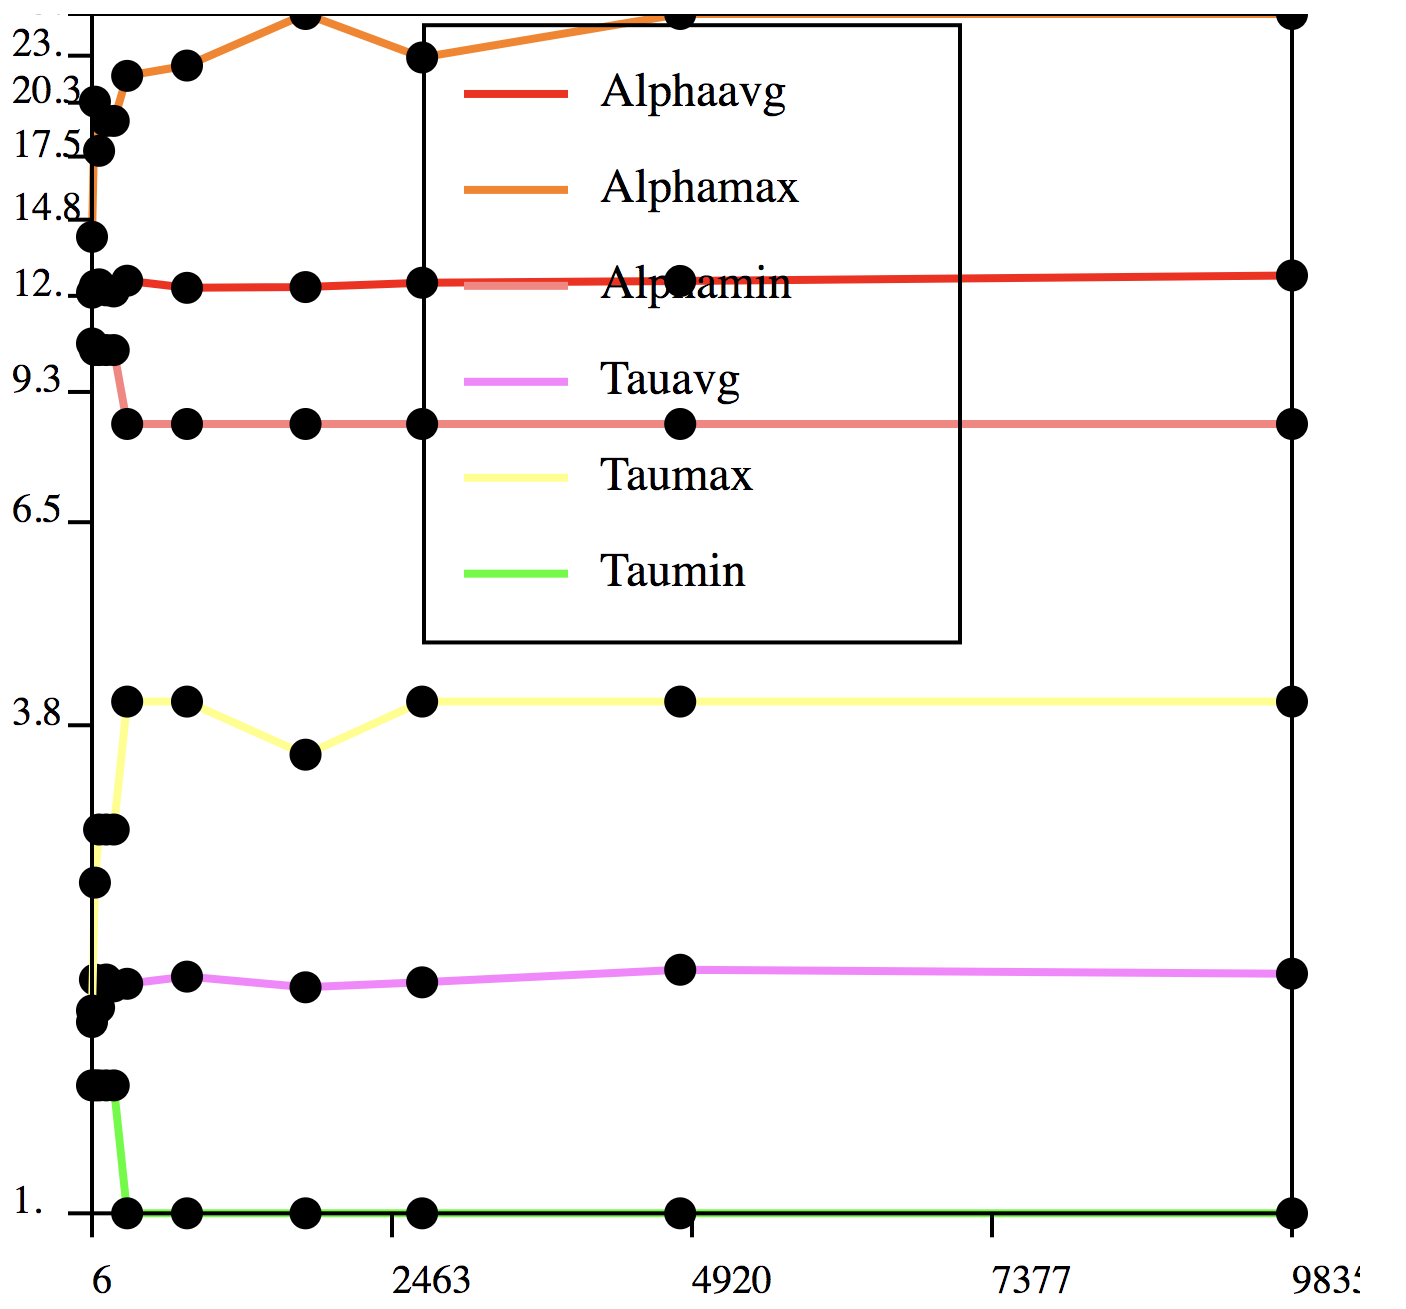
\includegraphics[width=0.48\linewidth]{figures/quality3} \hfill
	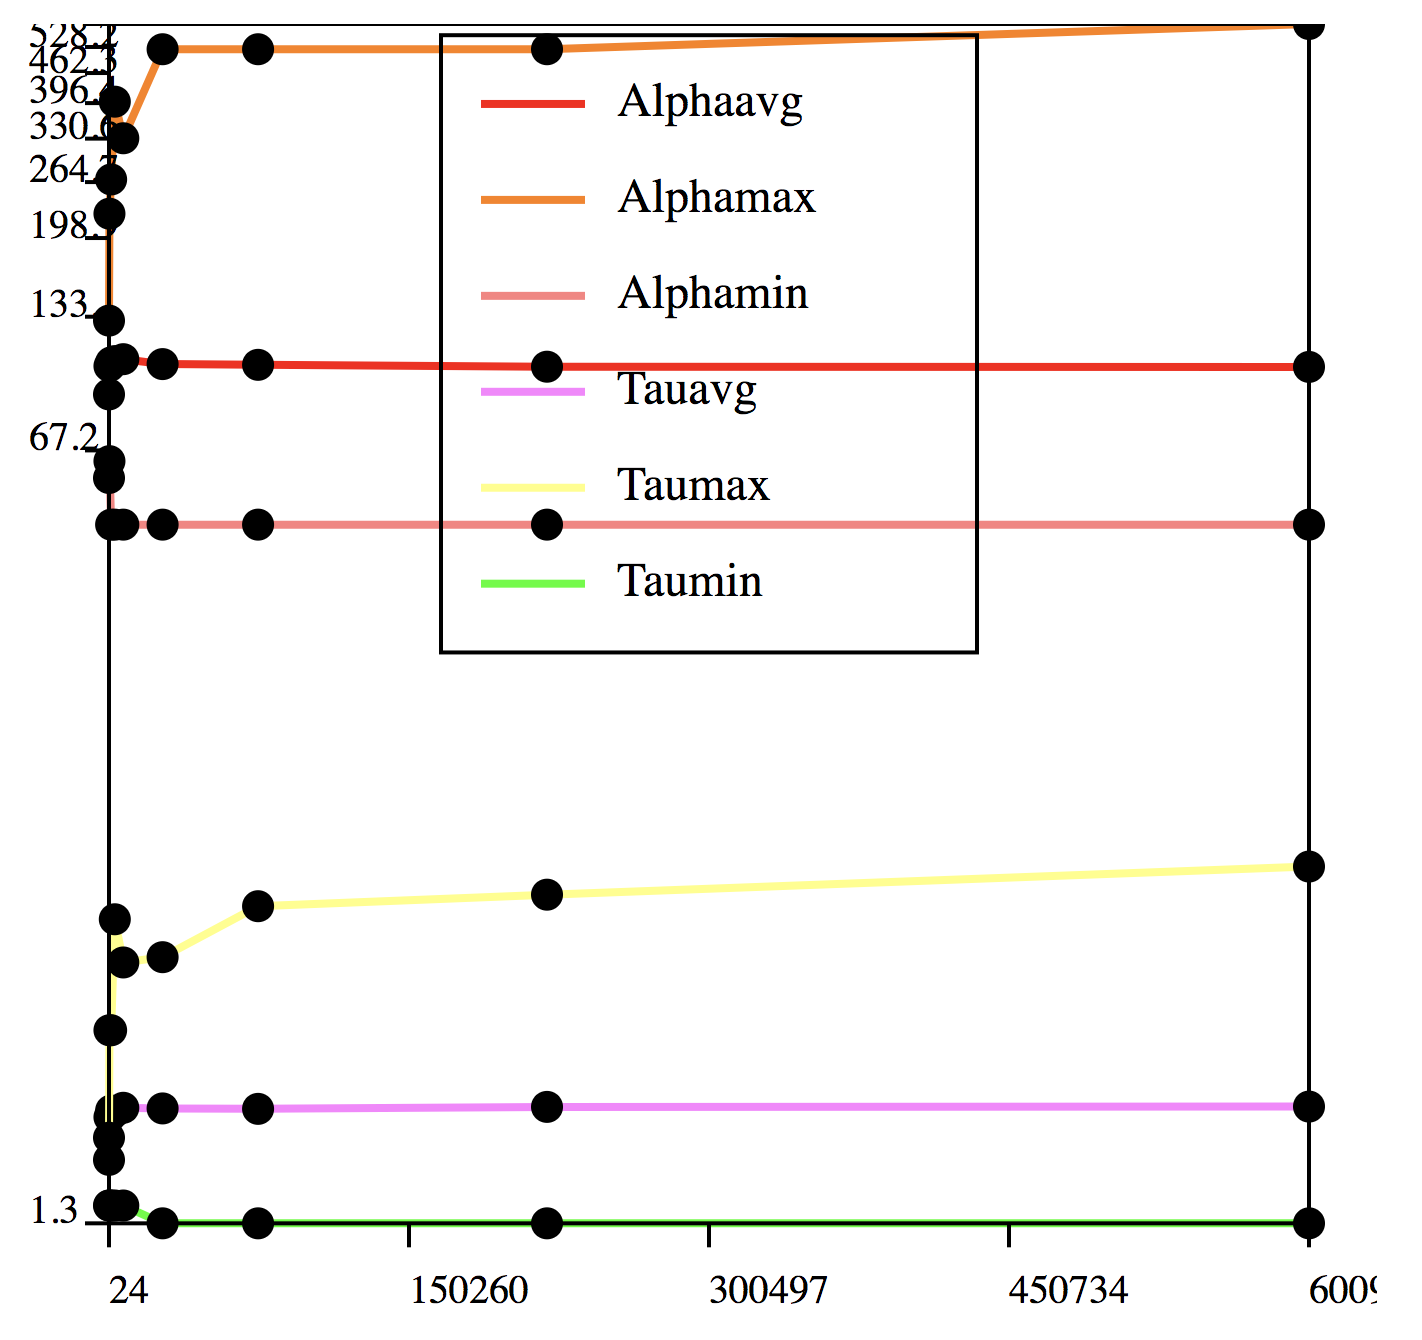
\includegraphics[width=0.48\linewidth]{figures/quality4} 
	\caption{Quality of the elements for several iterations of the adaptive refinement shown in Figure~\ref{fig:sphere}. The $x$ axis represent the total number of elements in the mesh. The $y$ axis the quality criterion (lower is better).
	 Left: 3D. Right: 4D.}
	\label{fig:quality}
\end{figure}

\begin{figure}[htbp]
	\centering
	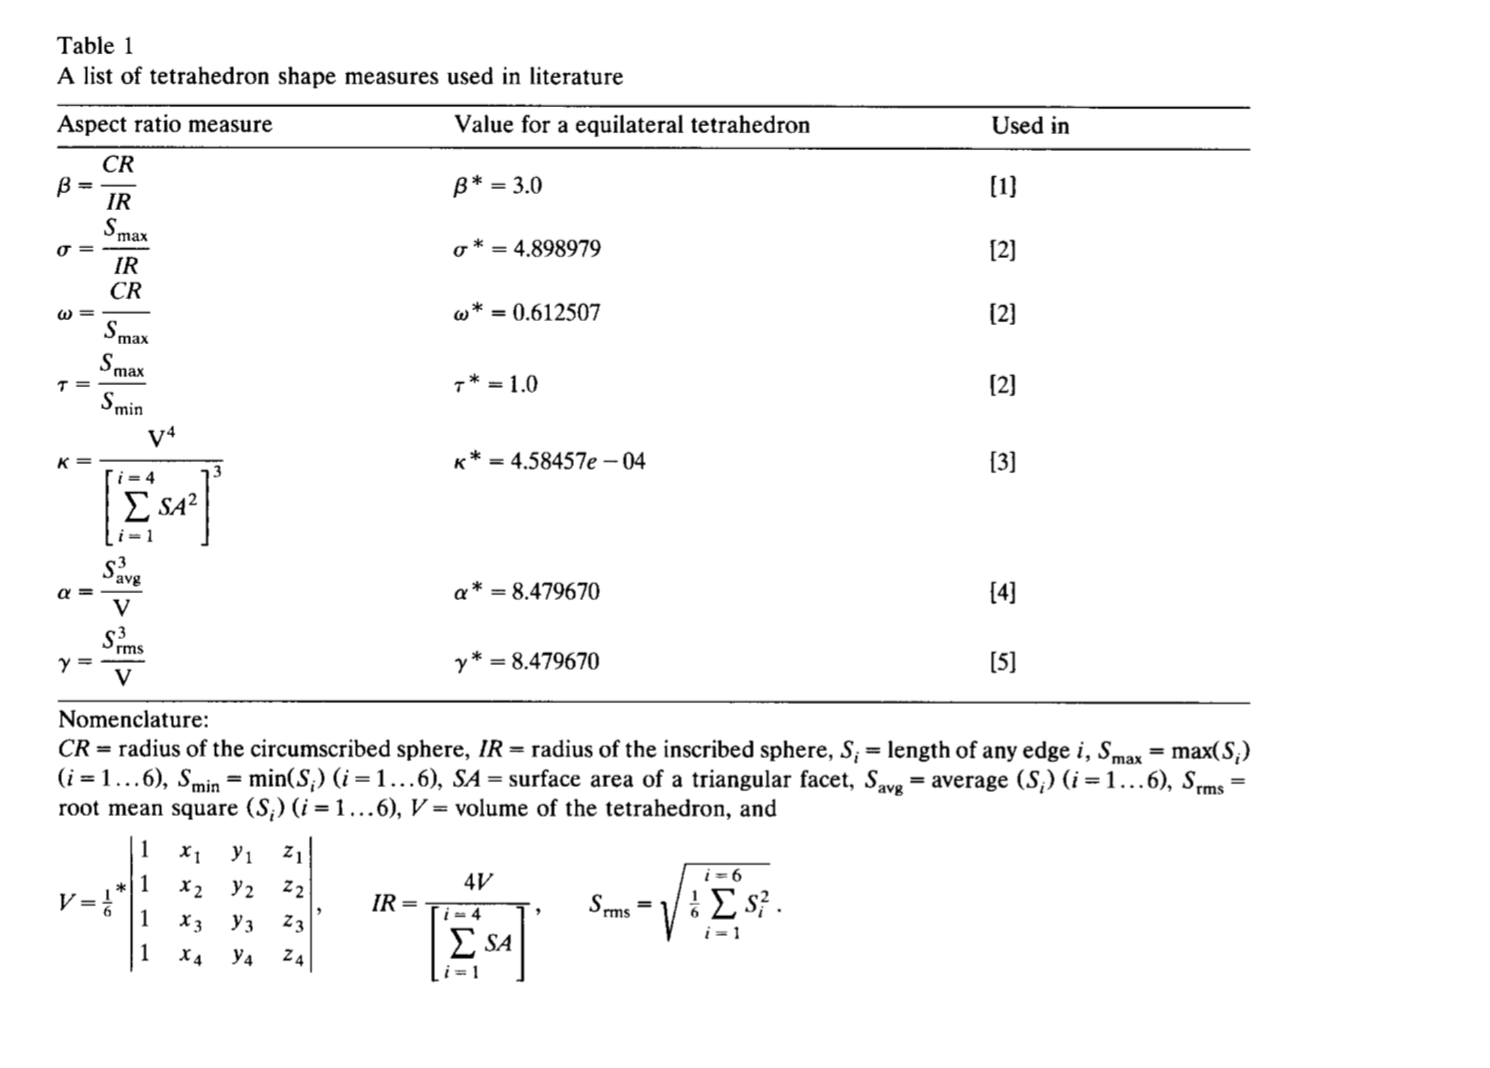
\includegraphics[width=0.8\linewidth]{figures/quality_metrics}
	\caption{Quality metics. We used ``Alpha'' and ``Tau''. }
	\label{fig:metrics}
\end{figure}



\clearpage

\section{Newest-vertex with longest edge for $D>2$}

Without a recurisve closure of the refined edge the overall element quality degrades very fast.

\begin{figure}[htbp]
	\centering
	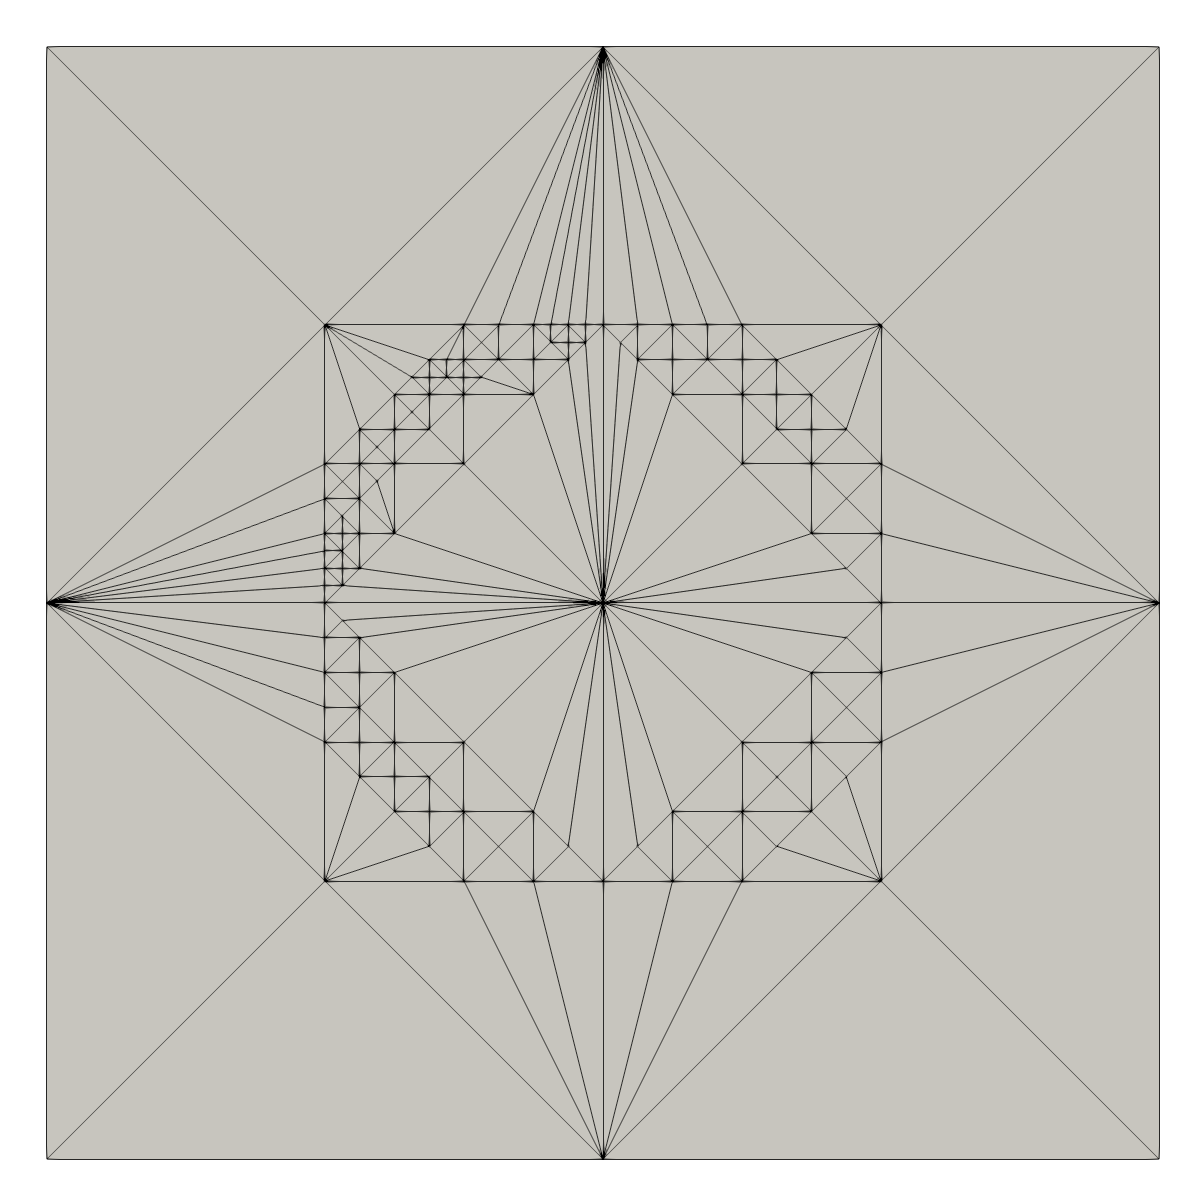
\includegraphics[width=0.48\linewidth]{figures/non-recursive} \hfill
	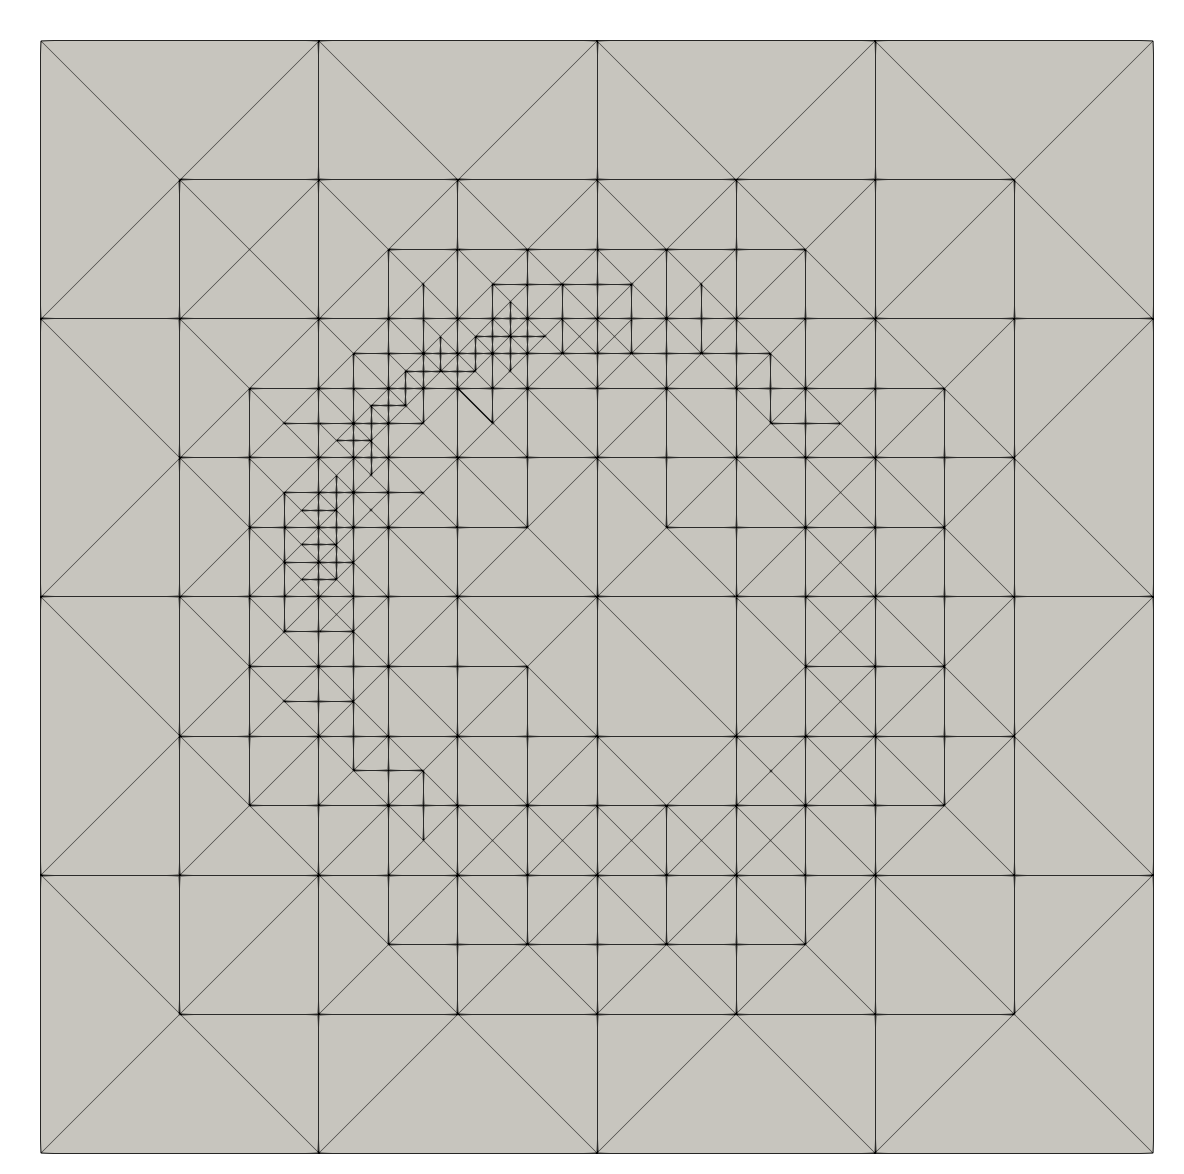
\includegraphics[width=0.48\linewidth]{figures/recursive}
	\caption{Non-recursive vs. recursive (3D).}
	\label{fig:metrics_r}
\end{figure}

\section{Quality of newest vertex with longest edge.}

While the longest-edge criterion is superior, the hybrid approach (newest vertex + longest edge) 
stays in the same order of magnitude for the degrading element quality. 
With further experiments it appears that the hybrid approach does not consistently generates conforming meshes.

\begin{figure}[htbp]
	\centering
	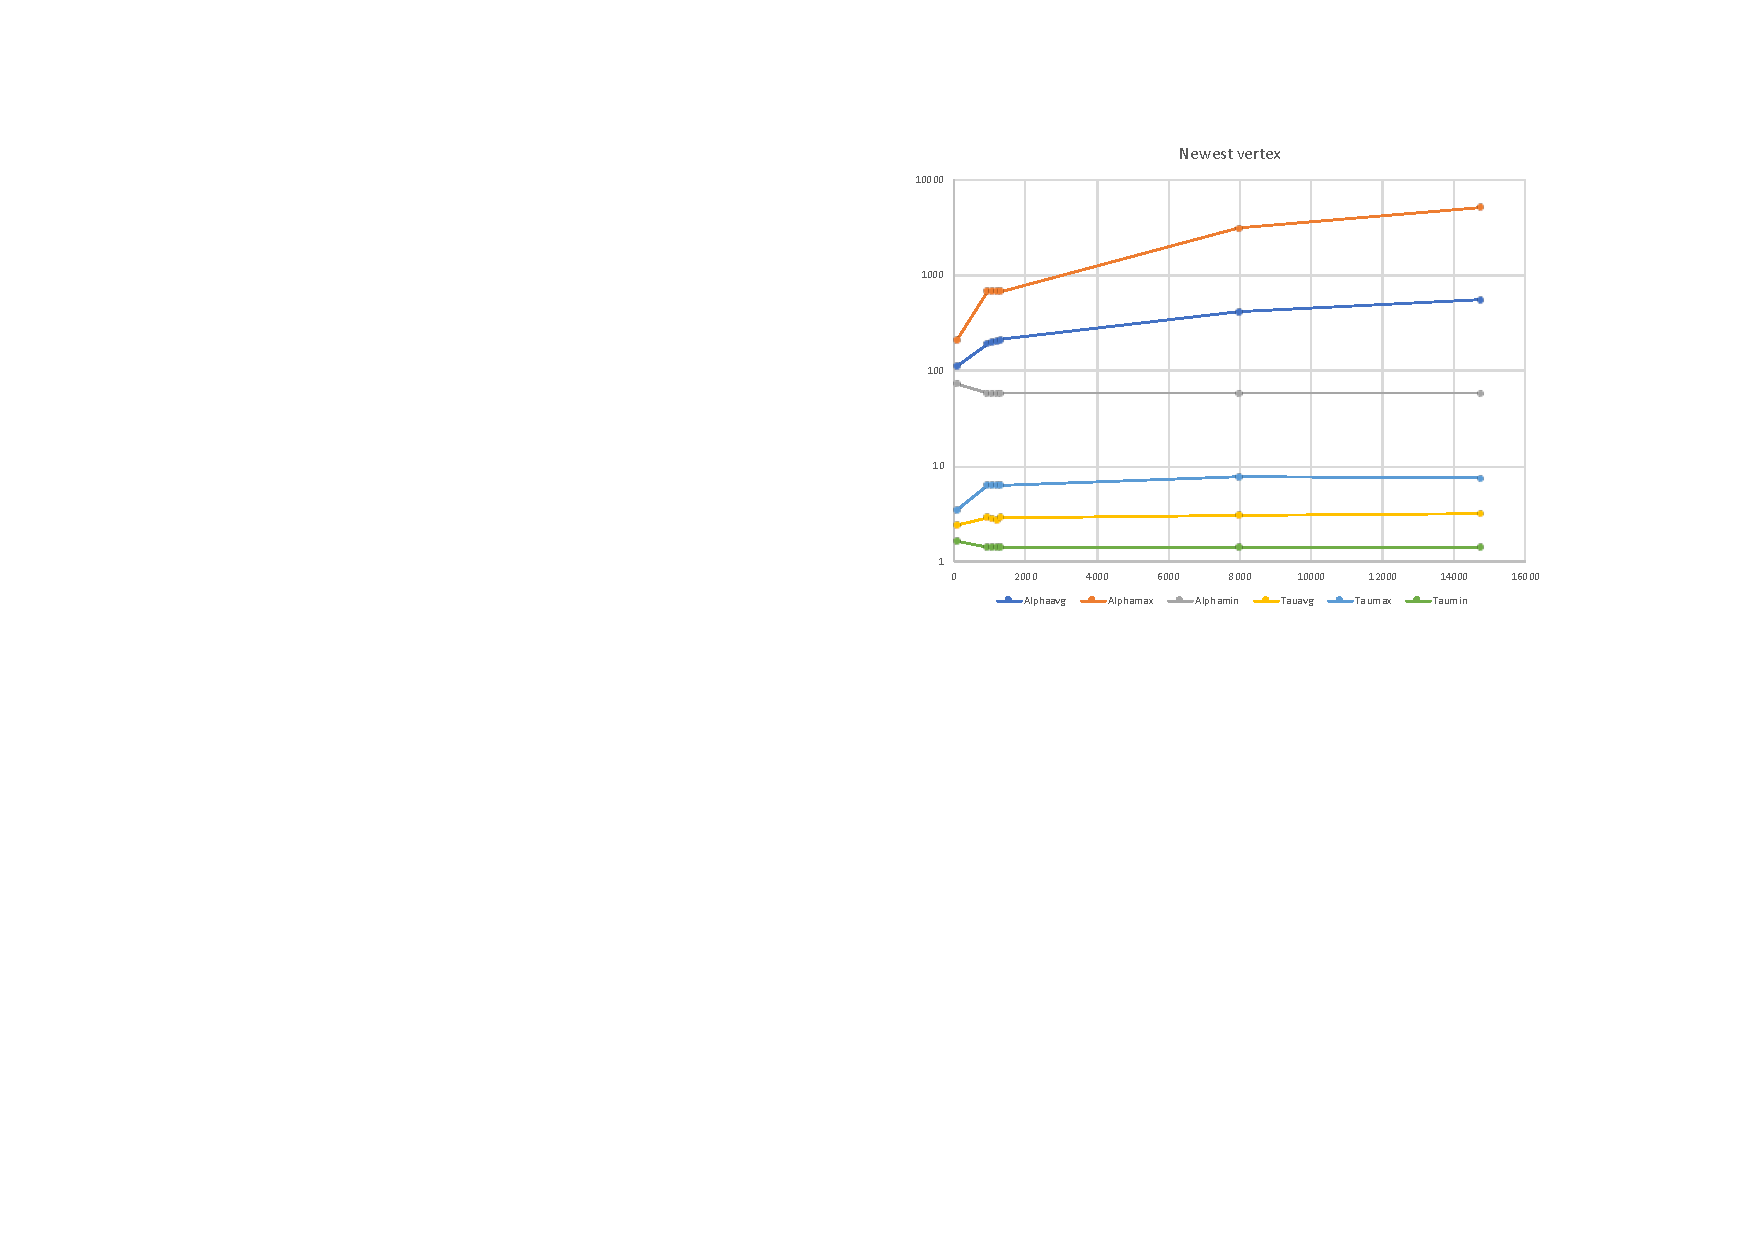
\includegraphics[width=0.48\linewidth]{figures/NewestVertex_Recursive} \hfill
	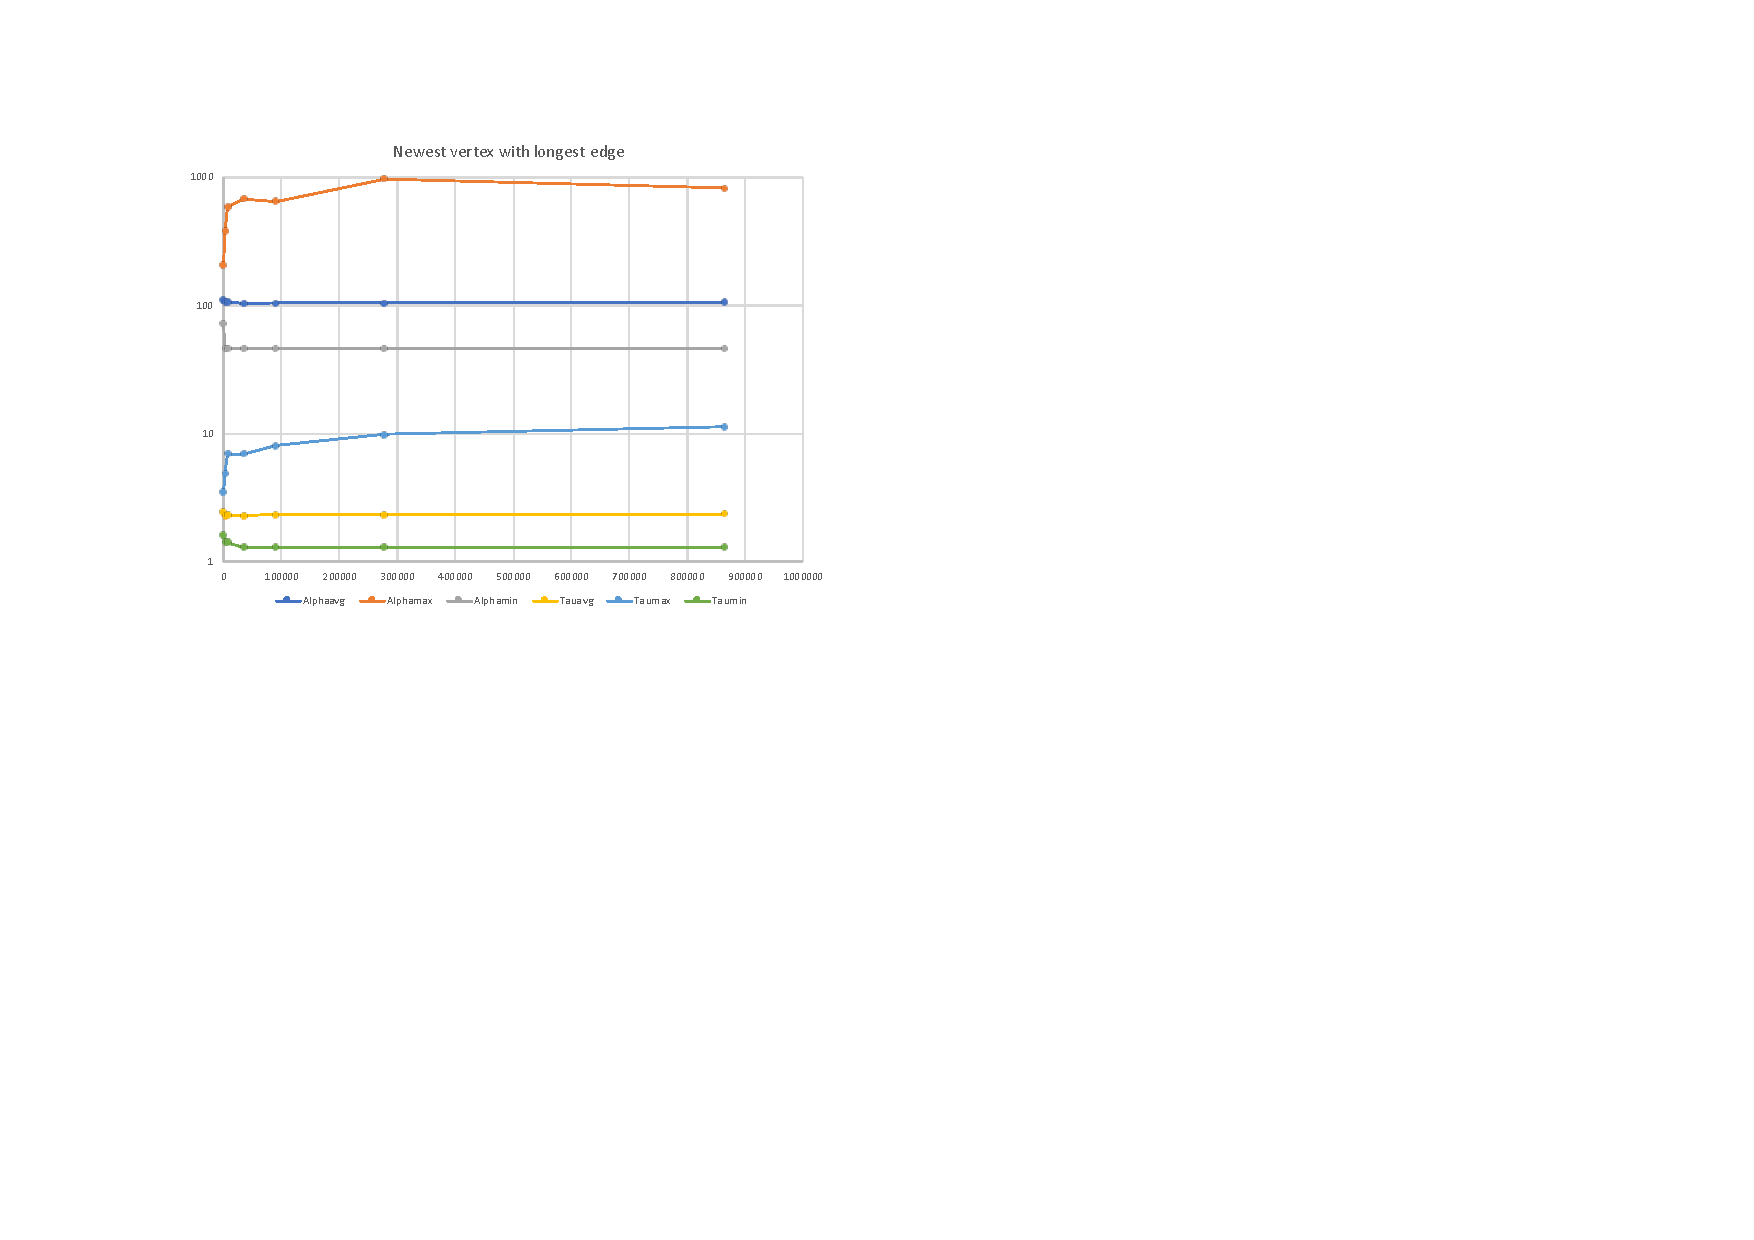
\includegraphics[width=0.48\linewidth]{figures/NewestVertex_and_LongestEdge_Recursive} 

	\caption{Quality of the elements for several iterations of the adaptive refinement shown in Figure~\ref{fig:sphere}. The $x$ axis represent the total number of elements in the 4D mesh. The $y$ axis the quality criterion (lower is better). The influence of longest edge shows on both the better quality and the larger number of elements generated.}
	\label{fig:quality_nv}
\end{figure}


\clearpage

\section{Parallelization}

Le $E$ be an element with vertex indices $I(E) = \{v_1, v_2, ... v_{D+1} \}$.

A way of producing a conforming mesh is to ensure that there exists only one sequence for refining an 
element and its facets. We call two neighboring simplices having a facet in common ``mates''.
Mates can be refined independently as long as the sequence of bisected edges is the same in their
common facet. 


The element refinement rule is based on the recursive longest-edge. However, the (rare) corner case where two edges have the exact same lenght is to be handled. For this reason we use the global identifier of the vertices of the mesh.
Let $e = (a, b)$ be and edge where $I(e) \subset I(E)$ $I_g(a), I_g(b)$ are global vertex identifiers and $I_g(a) < I_g(b)$. 

The set of edges associated with the element $E$ are sorted with respect to their length and lexicographically using $I_g(e)$. Hence, a facet is refined the same sequence of bisections for both the ``mates'' because the selection will be performed with the exact same order.

This implies that set $E$ can be split only once without requiring synchronization. Which leads us to the following parallel algorithm

\begin{enumerate}
	\item Mark elements for refinement
	\item Refine all marked elements and satisfy the compatibility chain as long as the elements in the chain have valid global indexing.
	\item $\Sigma$ is the edges for which the compatibility chain was not completed.
	\item Determine global identifiers for the newly added vertices (global communication) and communicate edges that have been bisected in the interface between two processes (point-to-point communication). 
	\item If $\Sigma \neq \emptyset$ mark the elements incident to each $e \in \Sigma$ and go to 2.
\end{enumerate}


\begin{figure}[htbp]
	\centering
	
\includegraphics[width=0.48\linewidth]{figures/partial} \hfill
	
\includegraphics[width=0.48\linewidth]{figures/complete} 

	\caption{Two steps of the parallel algorithm. Left: refinement of marked elements. Right: completion of the compatibility chain.}
	\label{fig:par_algo}
\end{figure}



\clearpage

% The parallel algorithm in 2D works by refinining independently the subdomains, then conforming the 
% interfacing edges (see Figure~\ref{fig:par_refinement}). 


%For D $>2$ this does not work since the faces might have been split diffrently because of the compatibility chain (recursive step).

% In higher dimensions the only local refinement strategy that seems to work well is newest-vertex bisection. 

% \begin{itemize}
% 	\item The inpendent set strategy
% 	\item \url{http://www.csc.kth.se/~jjan/transfer/bisect_0509.pdf}
% 	\item Coarsen and correct faces on the interfaces as in 
% \end{itemize}



% \begin{figure}[htbp]
% 	\centering
% 	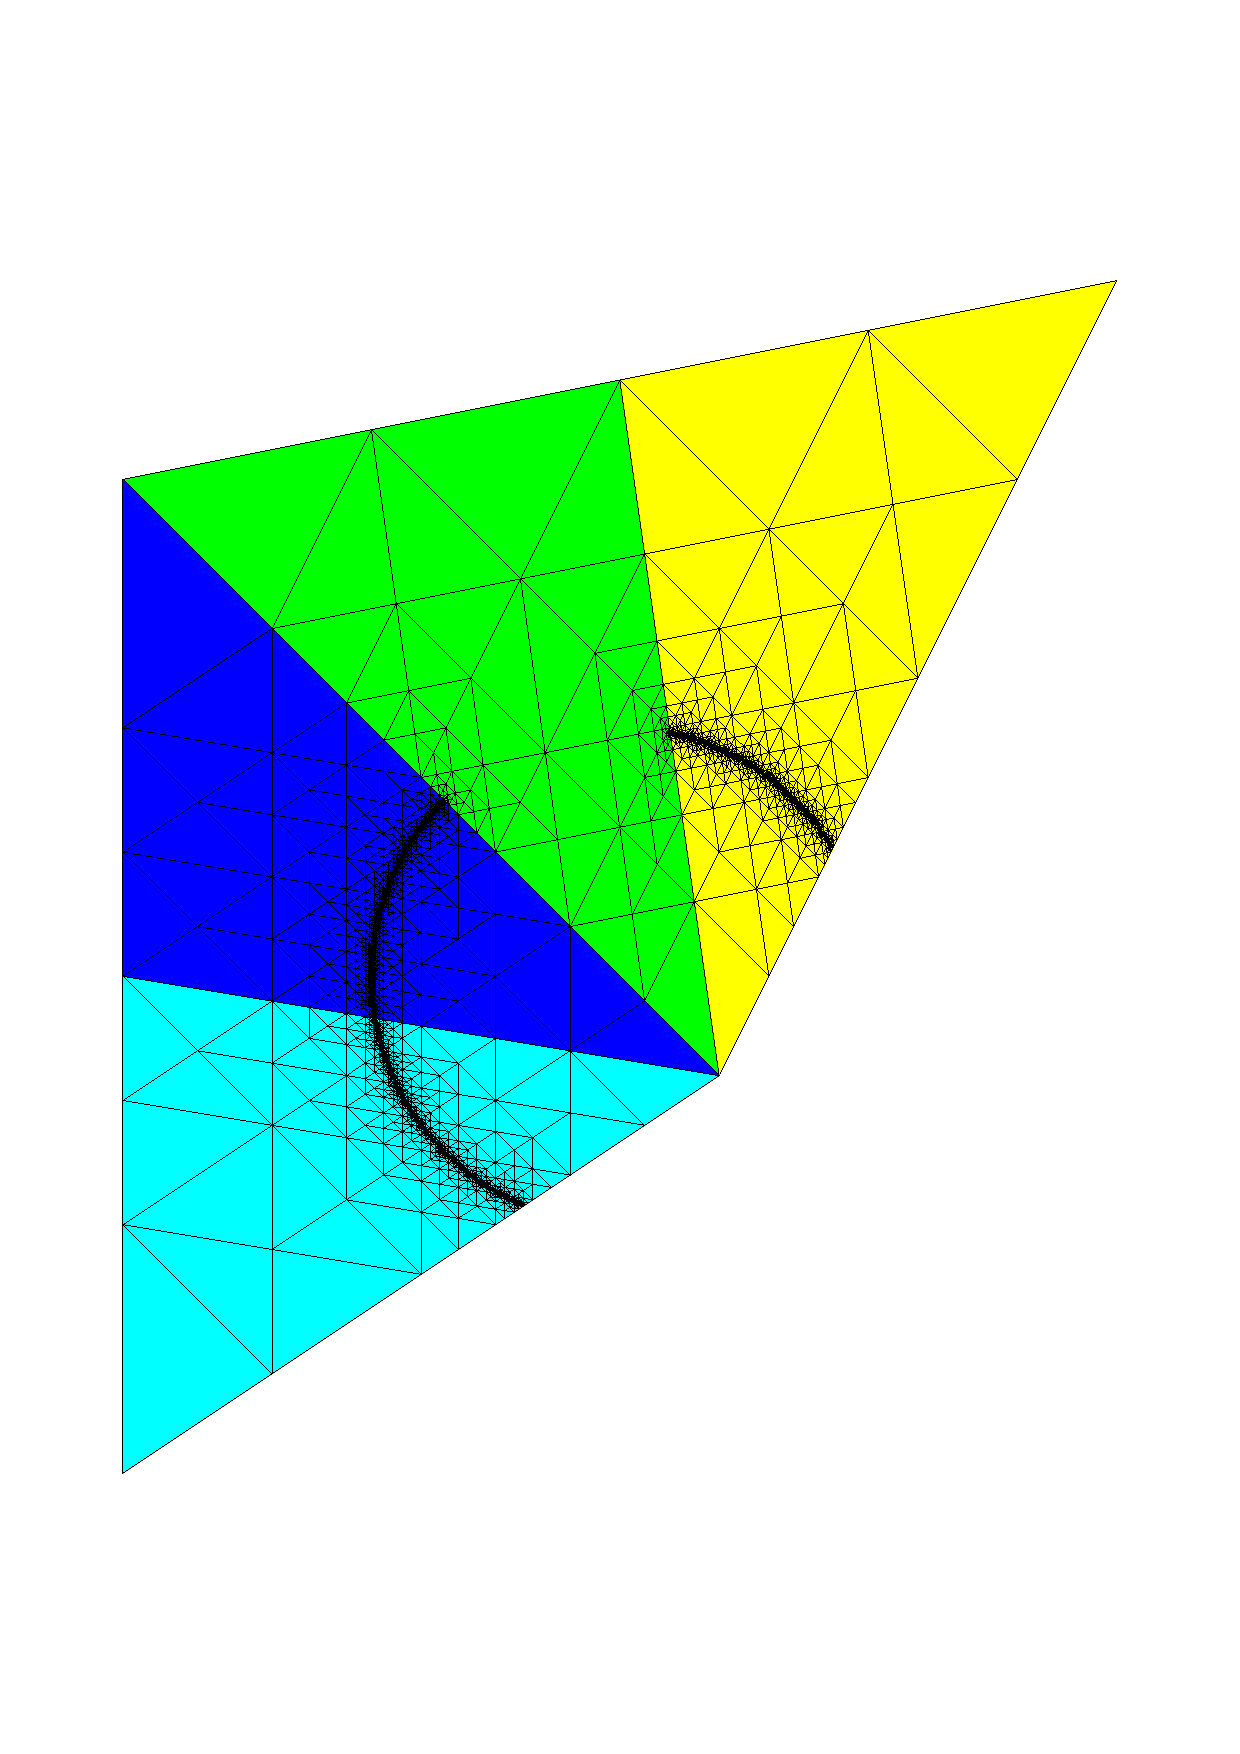
\includegraphics[width=0.48\linewidth]{figures/partitioning_with_one_part_without_refinement} \hfill
% 	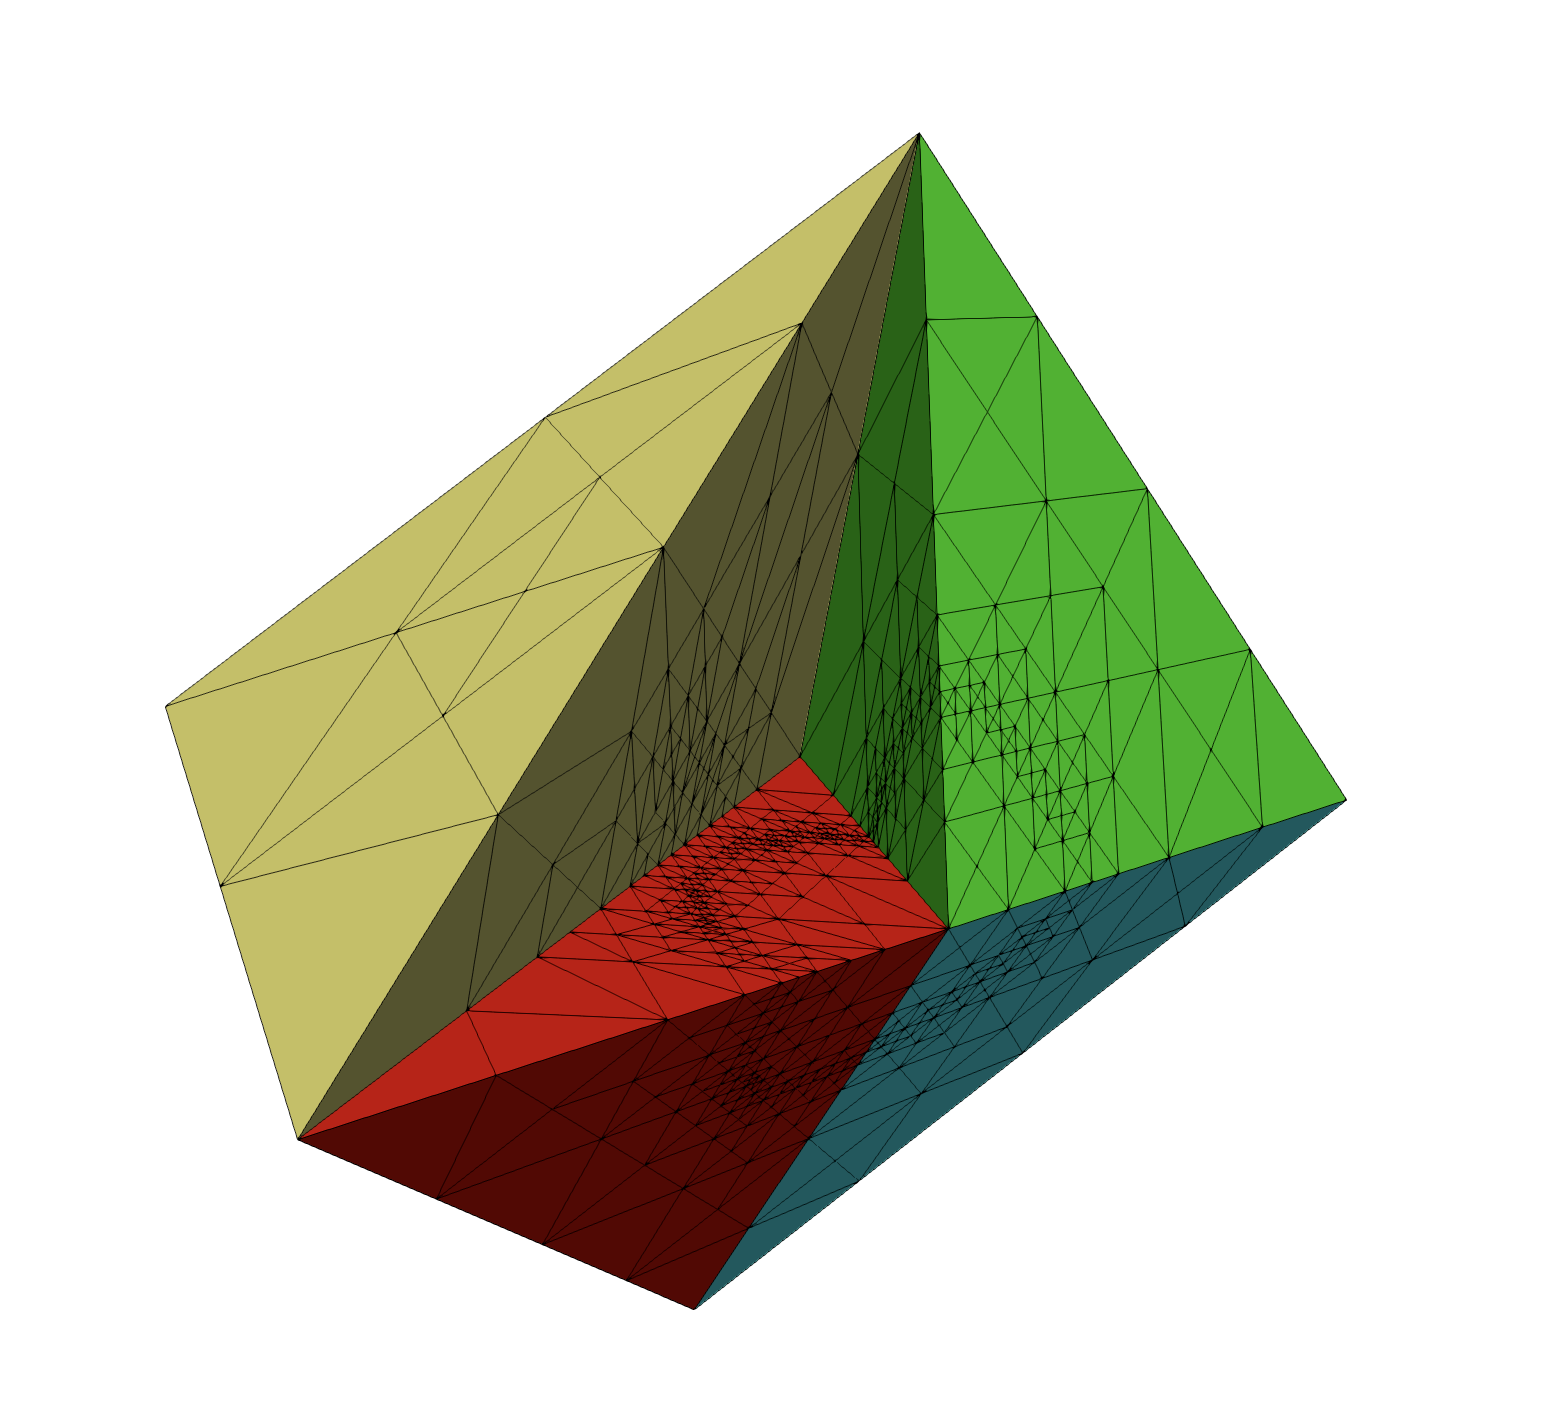
\includegraphics[width=0.48\linewidth]{figures/longest_edge}
% 	\caption{Partitioning with one part without refinement. Color represent partitions.}
% 	\label{fig:par_refinement}
% \end{figure}



\end{document}